\subsection{Brugeradministration}
\label{sub:Brugeradministration}

Brugeradministrationsmodulet har til opgave at kommunikere brugerdata mellem brugeren og databasen.

\subsubsection{Funktionalitet}
\label{ssub:Brugeradministration_funktionalitet}

Kommunikation mellem databasen og brugeren indebærer visning af information omkring en bruger, modtage inputs fra brugeren samt læse fra og skrive i databasen. At læse fra databasen indebærer, at den relevante information bliver hentet fra databasen, og vist på en acceptabel måde. Når der skrives til databasen menes der, at brugerens input bliver gemt i databasen. 

\subsubsection{Implementation}
\label{ssub:Brugeradministration_implementation}

\begin{figure}
  \centering
  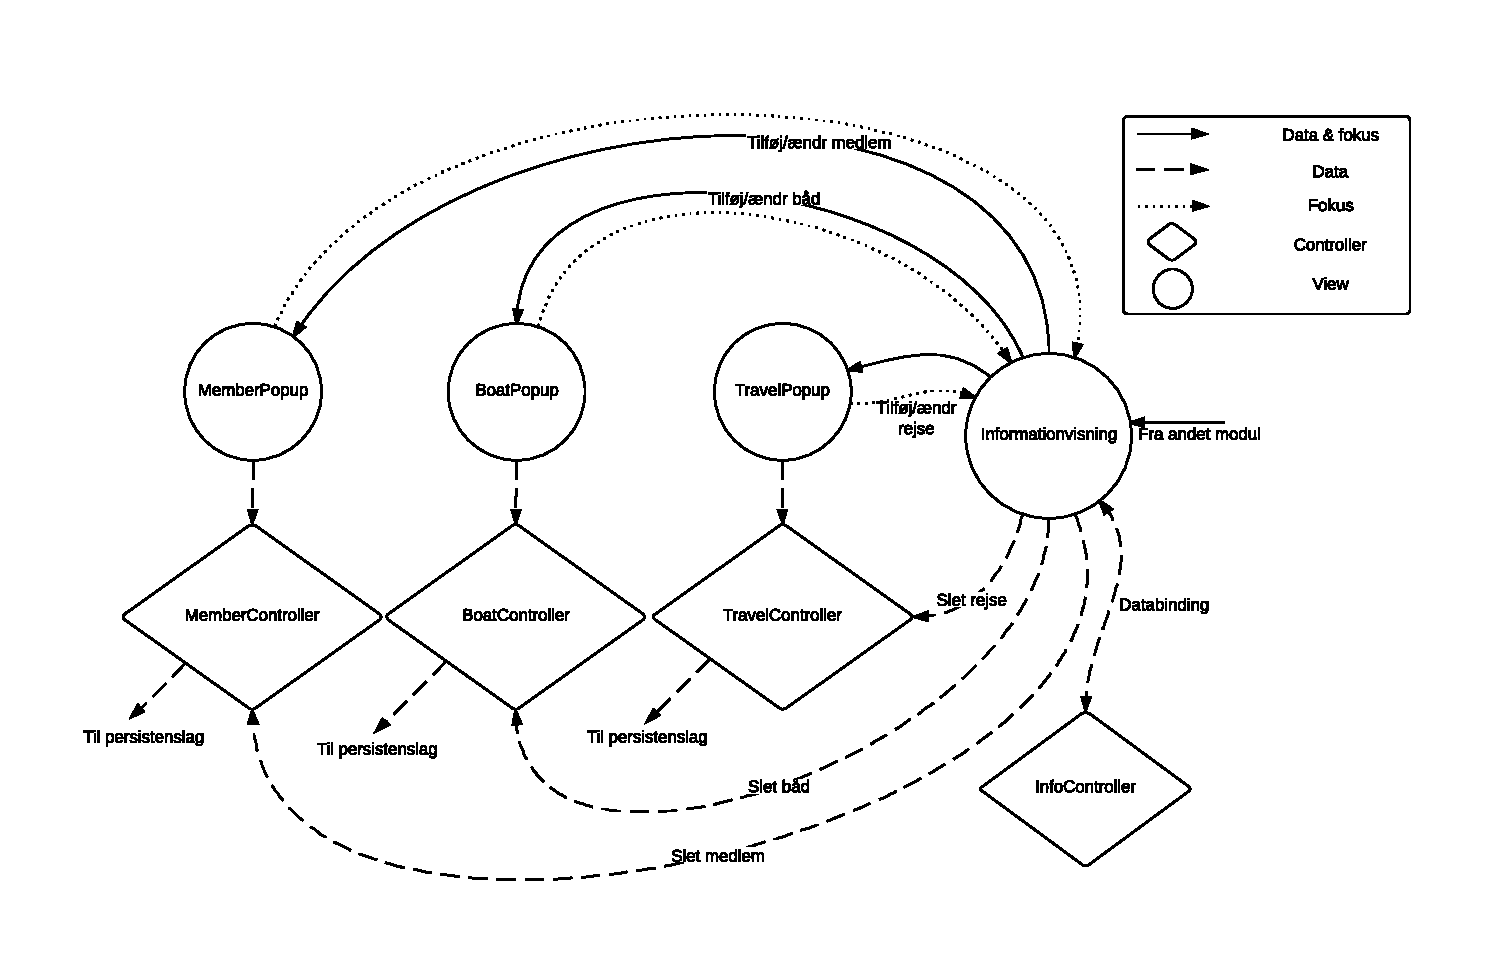
\includegraphics[width=\textwidth]{brugerinformation-diagram.pdf}
  \caption{Dette er tekst for tekst skyld}
  \label{fig:brugermod}
\end{figure}

For at implementere dette består brugeradministrationsmodulet af tre \enquote{popups} og fire \enquote{controllere}. Popups'ne og controllerne har parvis deres tilsvarende ansvarsområde som de sammen står for at bearbejde. Popup'erne tager brugerens input om tilføjelse og ændring af en bruger, og videregiver det til dens respektive controller. Controlleren kommunikere til persistenslaget som dernæst udfører brugerens ønskede handling. Popup'erne bruges kun til tilføjelse eller ændring af data. Dette gøres fordi der i brugerens situation skabes klarhed omkring, hvordan brugeren skal bære sig ad med at tilføje eller ændre data.

For at implementere dette består brugeradministrationsmodulet af et båd-, medlem- og rejse-delmodul. Delmodulerne har hvert deres tilsvarende ansvarsområde og er designet til at kunne læse, tilføje, redigere eller slette data fra databasen ud fra brugerens input. Læsningen af data foregår ved at et delmodul viser dets data i de respektive tekstfelter. For at redigere eller tilføje data, bliver der benyttet popup vinduer. Ved sletning af data markeres det ønskede elementer og der klikkes på fjern-knappen. Ved at bruge popup vinduer, kan brugeren lettere kan skelne mellem at læse data og skrive data.
